\documentclass{article}


\usepackage{amsmath}
\usepackage{amssymb}
\usepackage{enumerate}
\usepackage{fullpage}
\usepackage{bbm}

\def \mcX {\mathcal{X}}
\def \mcY {\mathcal{Y}}
\def \mcH {\mathcal{H}}
\def \mcD {\mathcal{D}}

\def \P {\mathbb{P}}

\def \N {\mathbb{N}}
\def \Nbr {\mathcal{N}}
\def \Q {\mathbb{Q}}
\def \F {\mathbb{F}}
\def \then {\implies &}
\def \oif {\Longleftrightarrow &\,}
\def \given {\text{Given }&}
\def \assume {\text{Assume }&}
\def \thfr {\therefore &\enskip}
\def \bij {\leftrightarrow}
\def \inj {\rightarrowtail}
\def \sur {\twoheadedrightarrow}
\def \Z {\mathbb{Z}}
\def \R {\mathbb{R}}
\def \C {\mathbb{C}}
\def \iff {\Longleftrightarrow}
\def \kron {\boldsymbol\delta}
\def \indicator {\mathbbm{1}}

\def\Tx{\textbf{x}}
\def\Ty{\textbf{y}}
\def\quotient{\mathclose{}/\mathopen{}}
\def\Tf{\textbf{f}}
\def\Th{\textbf{h}}
\def\Tg{\textbf{g}}
\def\sumn{\sum_{n=0}^\infty}
\def\limn{\lim_{n\rightarrow\infty}}
\def\prodn{\prod_{n=0}^\infty}
\DeclareMathOperator\adj{adj}

\newcommand{\stc}[1]{\widetilde{#1}}   
\newcommand{\pa}[1]{ \left({#1}\right) }
\newcommand{\set}[2]{ \left\{ #1 \,\middle|\, #2 \right\} }
\newcommand{\shift}[1]{&\quad & \text{#1}\\}
\newcommand{\lem}[1]{\text{\textbf{L.\ref{#1}}}}
\newcommand{\card}[1]{\left\vert{#1}\right\vert}
\newcommand{\Ps}[1]{\mathcal{P}\left({ #1 }\right)}
\newcommand{\colv}[1]{\begin{pmatrix} #1 \end{pmatrix}}
\newcommand{\mat}[1]{\begin{pmatrix} #1 \end{pmatrix}}
\newcommand{\detmat}[1]{\begin{vmatrix} #1 \end{vmatrix}}
\newcommand{\spanb}[1]{\text{span}\{ #1 \}}
\newcommand{\abs}[1]{\left|#1\right|}
\newcommand{\Inner}[1]{\langle #1 \rangle}
\newcommand{\Innercpy}[1]{\langle #1, #1 \rangle}

\DeclareMathOperator{\Err}{\text{err}}
\DeclareMathOperator*{\ErrE}{\mathbb{E}}
\DeclareMathOperator{\Tr}{tr}
\DeclareMathOperator{\Dim}{dim}
\DeclareMathOperator{\Rank}{rank}
\DeclareMathOperator{\Ker}{ker}
\DeclareMathOperator{\Diam}{diam}
\DeclareMathOperator{\Int}{int}
\DeclareMathOperator{\Clo}{clo}
\DeclareMathOperator{\sgn}{sgn}
\DeclareMathOperator{\MyRe}{Re}
\DeclareMathOperator{\MyIm}{Im}

\usepackage{graphicx}
\usepackage{float}
\usepackage{fullpage}


\title{Music Genre Classification\\\large COS424}
\author{Vladimir Feinberg, Siddhartha Jayanti}
\date{9 February 2016}

\begin{document}
\maketitle

\begin{abstract}

We explore a variety of supervised learning approaches for genre classification on an excerpt of the GTZAN dataset \cite{TC}. Methods explored are {\em Softmax, SVM, mSVM, Nearest Neighbors, Random Forest, Adaboosted Decision Stumps, Voting}, and a novel {\em Binary-Search mSVM} algorithm.
The top-performing method was an mSVM trained on the most informative 36\% of the \texttt{mfcc} and \texttt{chroma} features as determined by a Random Forest, a strategy used by \cite{vox}. This achieved 75.1\% with the features in Fisher vector representation, the hyperparameters of which where selected with a partial grid search.

\end{abstract}
 \section{Introduction}

A basic problem in supervised machine learning for audio data is to label a song into a genre such as blues, classical, country, disco, hip-hop, jazz, metal, pop, reggae, rock.
This problem is difficult because the representation of sound may translate into these genres in a nontrivial fashion.
Furthermore, a given song can have multiple genres - two people may disagree on its labelling even if they agree on a large set of other songs. This implies that even in nature the learning process for genre classification leads to inconsistent results. Thus, for a given labelling, it is difficult to expect there to be an arbitrarily accurate classifier.
Finally, any given pair of genres differ in amount of variation, with some being easier to distinguish than others.

We will explore a variety of supervised learning methods and evaluate their performance for the GTZAN dataset \cite{TC}.

\section{Data representation}

We work with a small version of the dataset, with 1000 songs, 100 for each genre. Each song is labelled with one of the aforementioned 10 genres.

\begin{center}
\begin{tabular}{ l | l }
  {\bf feature} & {\bf dimension}\\
  eng & $(1 \times f)$   \\
  chroma & $(12 \times f)$   \\
  t & $(1 \times f)$   \\
  keystrength & $(12 \times f)$   \\
  brightness & $(1 \times f)$   \\
  zerocross & $(1 \times f)$   \\
  roughness & $(1 \times f)$   \\
  inharmonic & $(1 \times f)$ \\
  hcdf & $(1 \times f)$  \\
  mfcc & $(32 \times f)$ \\
\end{tabular}
\end{center}

Though each of the songs was approximately 30 seconds in length, the precise number of frames in each song differed. Each was padded to $f = 1222$, the maximum number.

Thus, we had to either pad or chop the feature matrices to make them of equal dimension
for all songs.
We chose to pad the feature matrices of shorter songs with 0s as opposed to chopping longer songs
so that we would not lose any of the information in the final frames of longer songs.

\section{Previous Work}

The nature of the sound data includes many features which are not predictive of the labels - there is noise in the information-theoretic sense. Secondly, there are variations for songs within genres whose differences are present in the feature vectors for the individual clips, but these types of more subtle musical notes do not interest us.

An often-applied dimensionality reduction technique is PCA; however, its unsupervised nature makes the reduction uninformed with respect to predictive features \cite{WellingNote}.

Techniques in the aforementioned source are used on {\em timbre-related} musical features in Enrique et al. \cite{ERLGRR}. They obtain a $4.09\%$  error with \texttt{mfcc} and Fisher-LDA. A later paper by Chang et al. \cite{CJI10} uses both short and long term features of music and the compressive sampling technique to keep
the dimensionality low. They obtain $92.7\%$ accuracy on a different dataset. Note that these papers do not use the same GTZAN source, so their performance metrics do not directly carry over.

\section{Exploratory Feature Analysis}

Note from now on the labels are named according to their index in alphabetical order. For code that generated these files, see \texttt{exploratory-feature-analysis.ipynb}.

\subsection{MFCC}

The matrix representation for \texttt{mfcc} is large and inconvenient. Upon recommendation by the TAs (with their scripts as well), we used the Fisher vector (FV) representation for this data set. The representation takes two inputs: the number of clusters to use for its GMM model and the exemplar size to encode temporal info. As these parameters increase, the number of features in the FV does as well. When referring to a FV representation, we will mark these parameters in that order.

The FV computation seemed to exhibit a sort of periodicity. We can re-shuffle the indices of the FV to make each item in each period adjacent to one another. After noticing that these values are nearly identical (see Figure \ref{fig:fv33}), we decided to average them and only keep the average as a reduction by a factor of the innermost period.

\begin{figure}[H]
    \centering
    
    \begin{minipage}[b]{0.3\textwidth}
        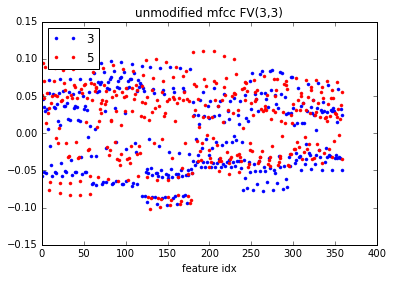
\includegraphics[width=\textwidth]{unmodified-mfcc3-3.png}
        %\caption{}
    \end{minipage}
    \hfill
    \begin{minipage}[b]{0.3\textwidth}
        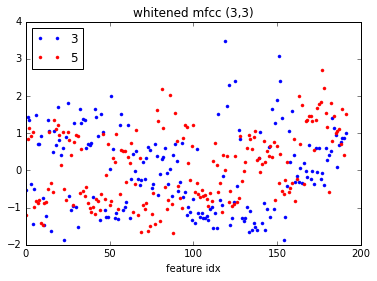
\includegraphics[width=\textwidth]{whitened-riffled-mfcc3-3.png}
        %\caption{}
    \end{minipage}
    
    \label{fig:fv33}
    \caption{Here we compare the FV for \texttt{mfcc} on two different labels. Note that for every outer period (of which there are 6) there exists an internal periodicity of 5 in this example, where bands form for every item.}
\end{figure}

The above example with \texttt{mfcc} FV(3,3) has equivalent performance in an example classifier - RBF-kernel based SVM with regularization constant 1, with 0.69 accuracy on a holdout test set for both the unmodified and reduced data.

This periodicity extends to other parameters as well - see for example the FV(8,5) case in the Appendix, figure (\ref{fig:fv85}). In addition, this holds for other types of features, not just \texttt{mfcc}.

In fact, 15 random pairs from the set of parameters $[10]\times[10]$ were examined (where $[n]$ is the set of integers $1, ..., n$) visually confirm an outer period of size $2C$ and inner period of size $t=2n-2(n\mod 2)-1$ for FV($C$,$n$).

Upon recommendation from a TA, we abandoned the periodicity approach because we were losing valuable information in the case where the ``bands" were not nearly identical in size.

However, this still points to an interesting direction in data representation in the future that may be more amenable to higher accuracies. One representation that was attempted (but it did not improve accuracy) was to keep the averages, and then append the differences of $t-1$ values in each period from the average of the entire $t$-sized period (this was done instead of just appending the average values to maintain the same number of degrees of freedom). There is room in the future to explore this representation.

Further attempts at dimensionality reduction included PCA, which did not demonstrate much potential - no single feature contributed to much of the explained variance, indicating that the high-dimensional space that the FV occupies is saturated by the data - there's no low-dimensional plane that the data lie on.

\begin{figure}[H]
    \centering
    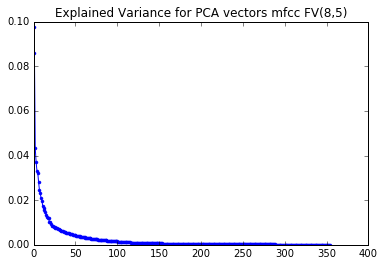
\includegraphics[scale=0.5]{pca-mfcc8-5.png}
    \label{fig:pca}
    \caption{Note that the most significant dimension only explains less than 0.1 percent of the variance
    in the data, and that the drop off is quite gradual.
    This indicates that the fisher vectors don't lie in a much smaller dimensional subspace.
    We also note that similar graphs can be generated for different parameter values of $C$ and $n$.}
\end{figure}


\subsection{Chroma}

Chroma also has a matrix representation. The FV-based analysis for \texttt{mfcc} was replicated for chroma features, yielding similar results.

Another line of analysis explored for chroma, but was not integrated into the classifiers, were kernel-based methods for imaging \ref{fig:chromakernels}.

\subsection{Already-vectorized features}

Other features were already in vector format, each of which had manageable sizes, and thus did not require any dimensionality reduction for tractability. Of these features, the inharmonic contained NaN values and thus was not considered further.

To quickly estimate how helpful these features would be in discriminating genre,
we ran random forest classifiers with each of them using depth 20 decision trees and 200 learners. The trees use the Gini coefficient for splitting and no pruning

\begin{center}
\begin{tabular}{l|c}
    {\bf Feature}   &   {\bf Accuracy} \\
\texttt{eng} & 0.381651 \\
\texttt{t} & 0.113942 \\
\texttt{brightness} & 0.303045 \\
\texttt{zerocross} & 0.332292 \\
\texttt{roughness} & 0.389904 \\
\texttt{hcdf} & 0.328526 \\
\texttt{mfcc} & 0.641907 \\
\texttt{chroma} & 0.507372 \\
\end{tabular}
\end{center}

We notice that the other features are not as helpful as \texttt{chroma} or \texttt{mfcc}, so we focus on these two instead.

\section{Methods and Performance}

\subsection{Operational notes}

\subsubsection{FV generation}

The provided MATLAB script was modified to be applied for chroma as well as \texttt{mfcc} data. A caching mechanism was used to prevent re-generation of FVs.

\subsubsection{Data Parallelism}

Both grid search and cross validation are embarrassingly parallel operations. Cross-validation was parallelized through internal \texttt{scikit-learn} multiprocessing. Hyperparameter search was parallelized through \texttt{python}'s \texttt{multiprocessing} for both laptop and cluster environments (in the case of the cycles servers, 4 terminals with 41 python processes each were launched for the largest grid search).

\subsection{Classification Methods}

Based on the initial experiments with the different features and the recommendations from the TAs, the \texttt{mfcc} features were used as a starting point.

\subsubsection{SoftMax}

Code: \texttt{exploratory-feature-analysis.ipynb}. To get an initial baseline for accuracy, we applied FV(3,3) in both \texttt{mfcc} and chroma form to a softmax regressor. Softmax is used instead of logistic regression for the multiclass selection because our labelling (unlike, possibly, in real life), each song belongs to only one genre.

We split the dataset into a 7:1 train:test holdout. On the training set, we use 8-fold cross validation to select the hyperparameter for the regularization coefficient. Then we re-learn the entire SoftMax model on the full training set, and apply it to the test set. This nested cv is used to avoid an inflated generalization error estimate caused by overfitting the hyperparameter to a holdout set.

\begin{figure}[H]
    \centering
    
    \begin{minipage}[b]{0.4\textwidth}
        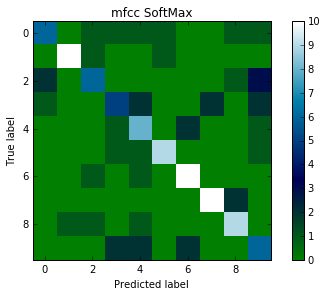
\includegraphics[width=\textwidth]{softmax-mfcc.png}
        \caption{\texttt{mfcc} holdout accuracy was 0.658, its training accuracy was 0.906}
    \end{minipage}
    \hfill
    \begin{minipage}[b]{0.4\textwidth}
        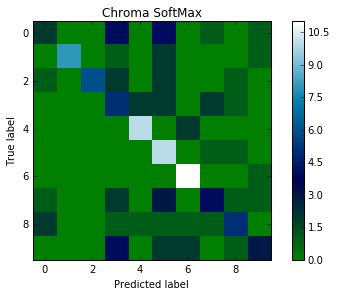
\includegraphics[width=\textwidth]{softmax-chroma.png}
        \caption{Chroma holdout accuracy was 0.533, training was 0.864.}
    \end{minipage}
    
    \label{fig:softmax}
\end{figure}

Both the \texttt{mfcc} and chroma softmax classifiers show a large drop from training to test accuracy, indicating a bias problem. This needs to be solved by a simpler model - because we used cross-validation to select the regularization parameter and there was still overfitting, we need to more intelligently select our features to encourage sparsity in our estimators. Unfortunately, this means turning to other classifiers - while the $\ell_2$ penalty was used, there was no support for the $\ell_1$ as a direct measure to alleviate this problem.

Luckily, it seems that chroma and \texttt{mfcc} have complimentary confusion matrices, which makes us optimistic about combining the two.

\subsubsection{Random Forest}

Code: \texttt{fv-randomforest.ipynb}. After trying boosted decisions stumps (see section \ref{boostedstumps} in the Appendix), it became clear that decision trees needed some depth to identify songs well. We switched using random forests to classify music instead - by enabling a more expressive decision tree, the weak learner can actually weakly specialize for a certain set of examples. Then the ensemble can use their specialization to have higher accuracy.

We ran 8-fold cross validated testing on the \texttt{mfcc} FV$(3, 3)$ vectors and optimized
the hyper-parameters {\em max-depth} of trees and number of {\em learners}.
The best accuracy we got was $65.7\%$ and the parameter values were $\textit{max-depth} = 20$  and $\textit{learners} = 900$.

As mentioned in the Already-vectorized features section,
we also performed random forest classification using some of the other features.
These classifications were done solely for the purpose of getting a rough estimate
of how well the features helped classify genre so that only the good ones could
be used in our meta-classification algorithm.
Therefore, the accuracies in the table in that section were obtained using
a one-shot 90-10 training-test split.
None of these accuracies broke even 40\%, suggesting to us that using any of the features
alone could not improve our overall accuracy.

\subsubsection{Nearest Neighbors}
Code: \texttt{fv-nearestneighbors.ipynb}.
Randomized forest attempts to make multiple feature-by-feature decisions to conclude,
while mSVM tries to use linear separators.
We used $k$-nearest-neighbors as a supervised learner that would work well if the FV(3, 3) data was clustered.
Once again, we used 8-fold stratified cross validation.
We stuck to Euclidean distance, and optimized the hyperparameter $k$ in the range $1 < k < 20$.
The best accuracy we got was $65.5\%$ for $k = 14$.

\subsubsection{Multi-class SVM}

Note in the below we don't have an external cross-validation loop as we do in SoftMax because of time constraints.

Code: \texttt{fv-msvm.ipynb}. The mSVM was the most promising across a variety of features. 8-fold stratified cross-validation for each parameter in a grid search of hyperparameters was performed (regularization coefficient $C$ on a 10-point log scale from -5 to 4, one-vs-one [ovo] and one-vs-rest [ovr] multiclass selection, and kernel type).

Kernels considered were RBF, polynomial $\kappa(\Tx_1, \Tx_2)=\pa{\gamma\Inner{\Tx_1,\Tx_2}+1}^{10}$ with $\gamma=\dim \Tx$, and linear. The choice of exponent for the polynomial kernel was made by visual inspection of the FV(3,3) case on \texttt{mfcc} until CV accuracy did not improve.

\begin{figure}[H]
    \centering
    
    \begin{minipage}[b]{0.4\textwidth}
        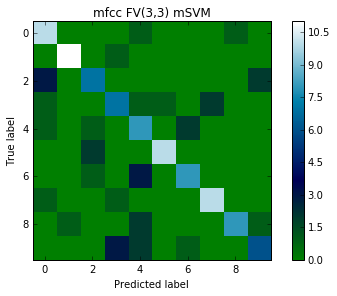
\includegraphics[width=\textwidth]{msvm-mfcc3-3.png}
        \caption{For \texttt{mfcc}, the optimal setting $C=100$, ovo, and polynomial kernel had 0.674 accuracy.}
    \end{minipage}
    \hfill
    \begin{minipage}[b]{0.4\textwidth}
        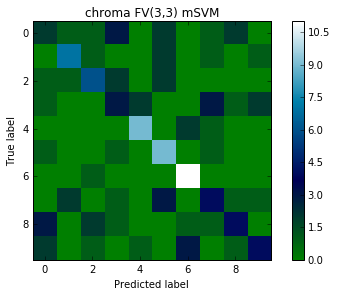
\includegraphics[width=\textwidth]{msvm-chroma3-3.png}
        \caption{For \texttt{chroma}, the optimal $C=1000$, ovo, and polynomial kernel had 0.475 accuracy.}
    \end{minipage}
    \label{fig:mSVM}
\end{figure}

The grid search ranges proved sufficient since none of the selected values were at the extremes. We note as in SoftMax the confusion matrices (From a 7:1 fold) are complimentary.

Going off this instinct, we appended \texttt{chroma} to \texttt{mfcc} and ran the same grid search. Indeed, accuracy improved to 0.684, with the same hyperparameters as the optimal for \texttt{mfcc} FV(3,3). We replicated this analysis for whitened data, but accuracy worsened, so we abandoned normalization. This is most likely due to the feature scales being representative of feature importance.

Exploring FV(8,8) with the same grid, we find \texttt{mfcc} at accuracy 0.682 with ovo, RBF, and $C=10000$; \texttt{chroma} at 0.516 with ovo, polynomial, and $C=1000$; and \texttt{mfcc+chroma} at 0.709 with ovo, polynomial, and $C=1000$.

At this point, for faster iteration, we only considered the grid with ovo and polynomial kernel. Furthermore, the log scale was switched to integers from 0 to 9. This seems justified based on the majority of optimal parameters so far. The introduction of \texttt{chroma} helps across FV sizes, but introduces lots of noise - now distances are increased even in features that ``might not matter" (at FV(8,8), there are 9152 columns). To combat this issue, we adopt an approach proposed in \cite{vox}: use Random Forests to identify most important features for classification (of concatenated \texttt{mfcc+chroma} vector), then train the SVM on only those features. We choose forests with 200 estimators and 20-depth trees as before. See Figure \ref{fig:rf-cutoff} for details.

\begin{figure}[H]
    \centering
    
    \begin{minipage}[b]{0.4\textwidth}
        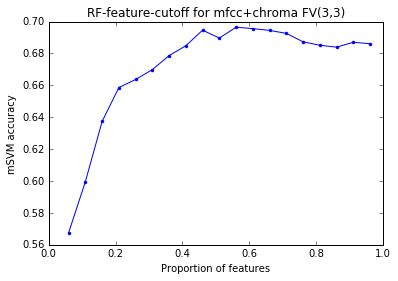
\includegraphics[width=\textwidth]{RF-cutoff3-3.png}
    \end{minipage}
    \hfill
    \begin{minipage}[b]{0.4\textwidth}
        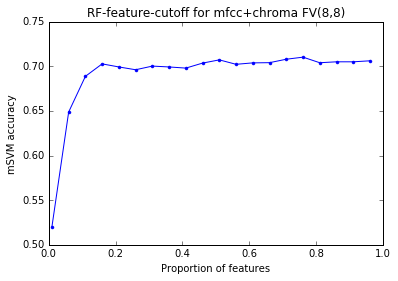
\includegraphics[width=\textwidth]{RF-cutoff8-8.png}
    \end{minipage}
    \label{fig:rf-cutoff}
    \caption{Using the RF to rank the features by importance and training the SVM on only a proportion of those parameters, we can see how the SVM's test error improves over feature quantity. In certain cases, the overfitting is apparent, with accuracy decreasing as the less important features are added.}
\end{figure}

We ran a parallelized grid search, over the grid of various combinations of exemplar and cluster sizes for both \texttt{chroma} and \texttt{mfcc}. Exemplar sizes considered were $\le 11$, and cluster counts were under 30. The full $(11\times 30)^2$ grid was not explored, only selections that we had time to generate (see code for details). For each FV configuration, for each regularization coefficient, an 8-fold cross validation was run, where every training set was used to learn the important features alone, and the same set was used to train the SVM. The top coefficient's average cv score is reported. Code: \texttt{explore-rf-svm.py}.

The proportion of features used was started off at 1\%, then increased by 5\% until the accuracy fell two times in a row. The results of the entire grid search are available in the repository.

The top configuration (at the time of the writing of this report) found was \texttt{mfcc} FV(9, 3) with \texttt{chroma} FV(20,11), resulting in accuracy 0.751, with 36\% of the features selected.


\begin{figure}[H]
    \centering
    
    \begin{minipage}[b]{0.4\textwidth}
        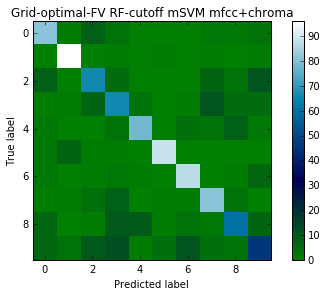
\includegraphics[width=\textwidth]{final-confusion.png}
    \end{minipage}
    \hfill
    \begin{minipage}[b]{0.4\textwidth}
        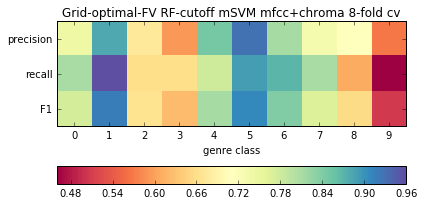
\includegraphics[width=\textwidth]{prf.png}
    \end{minipage}
    \label{fig:finalconf}
    \caption{The confusion matrix illustrates the low scores for the precision and recall with genres 3 and 9 - clearly, they are being confused for one another. Rock and country are indeed difficult to distinguish in some cases, even for humans.}
\end{figure}

Note that FV parameter selection is done outside the cv loop. A nested cv is not computationally tractable. However, since the FVs were selected to determine the data representation, the overfitting that's achieved with them is arguable. Also, the grid search was not run to completion becuase of time constraints.

\subsubsection{Other methods}

Please see the Appendix for other methods, including majority voting over different features (Section \ref{majority-features}) and Convolutional Neural Networks (Section \ref{cnn}). Unfortunately, none of these performed better than the above-mentioned classifiers.

\section{Conclusion}

We have applied a variety of methods to the genre classification problem. The top performer was RF-based feature selection for mSVMs on FV-encoded \texttt{mfcc} and \texttt{chroma} data.

There are different things to try out which may improve accuracy. As mentioned earlier, there is periodicity to exploit in the Fisher vectors. A representation which better captures the types of changes that occur within and between the FV periods may improve performance for all classifiers. For instance, it might be worth using the parameters for a parabolic fit to each period (this would be two values instead of $t$, but would still capture temporal differences).

Similarly, it would be worthwhile to investigate whether the high-dimensional data (both \texttt{mfcc}, chroma, and the other vectors considered) lie in a low-dimensional submanifold of their high-dimensional space - Isomap and Locally-linear embedding would be two approaches that help with this.

We made heavy use of \texttt{iPython} \cite{iPython} notebooks, \texttt{sklearn} \cite{scikit-learn} for algorithm implementations, \texttt{scipy} \cite{scipy} for scientific computing, and \texttt{matplotlib} \cite{matplotlib} for graphing.

Finally, we would like to acknowledge the assistance of the COS424 Spring 2015 TAs, both in providing advice and the initial FV scripts used. Finally, the Princeton University Computer Science Department's \texttt{cycles} cluster was used for parallelized grid-search. This facilitated much faster exploration of the large amount of FV parameters. 
\pagebreak

\bibliographystyle{acm}
\bibliography{bibliography}

\pagebreak
\section{Appendix}

\subsection{Additional Images}

\begin{figure}[H]
    \centering
    
    \begin{minipage}[b]{0.4\textwidth}
        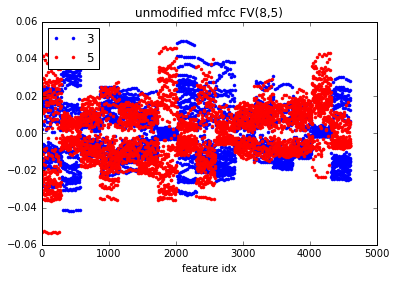
\includegraphics[width=\textwidth]{unmodified-mfcc8-5.png}
        %\caption{}
    \end{minipage}
    \hfill
    \begin{minipage}[b]{0.4\textwidth}
        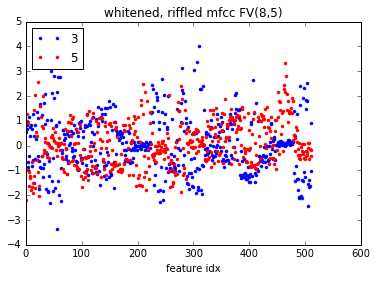
\includegraphics[width=\textwidth]{whitened-riffled-mfcc8-5.png}
        %\caption{}
    \end{minipage}
    
    \label{fig:fv85}
    \caption{
Learning with mSVM with the unmodified fisher vectors led to 67\% accuracy
while learning on the reduced vectors led to 68\% accuracy,
further confirming that no significant amount of information was lost by reducing
the dimension.}
\end{figure}


\begin{figure}[H]
    \centering
    
    \begin{minipage}[b]{0.3\textwidth}
        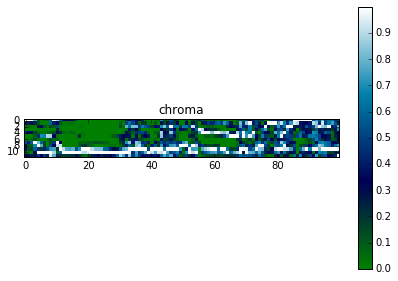
\includegraphics[width=\textwidth]{chroma-bare.png}
        %\caption{}
    \end{minipage}
    \hfill
    \begin{minipage}[b]{0.3\textwidth}
        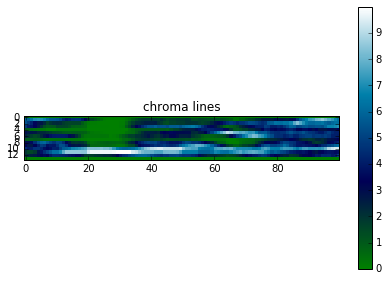
\includegraphics[width=\textwidth]{chroma-lines.png}
        %\caption{}
    \end{minipage}
    \hfill
    \begin{minipage}[b]{0.3\textwidth}
        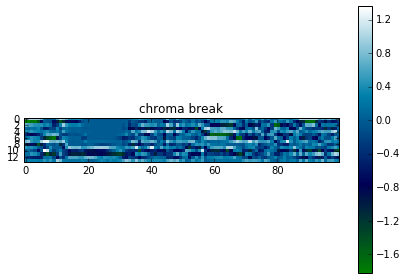
\includegraphics[width=\textwidth]{chromc-line-end-.png}
        %\caption{}
    \end{minipage}
    
    \label{fig:chromakernels}
    %\caption{    }
\end{figure}

    Chroma seems to be defined by long streaks of high values in otherwise sparse data. Two kernels which accentuate these effects would be the ``line kernel" - which is just a matrix with horizontal band of ones, and matrix that detects the beginning of such lines - ``chroma break" uses $\mat{0&0&-1\\0&0&+1\\0&0&-1}$

\subsection{Unsuccessful Classification Attempts}

\subsubsection{Boosted Decision Stumps}\label{boostedstumps}

Code: \texttt{fv-decisionstumps.ipynb}. Using AdaBoost on Decision Stumps (using Gini coefficient for selection), the FV(3,3) \texttt{mfcc} data performed poorly, failing to breach 26\% accuracy. 8-fold stratified cross-validation was used over the entire data set.


\begin{figure}[H]
    \centering
    
    \begin{minipage}[b]{0.4\textwidth}
        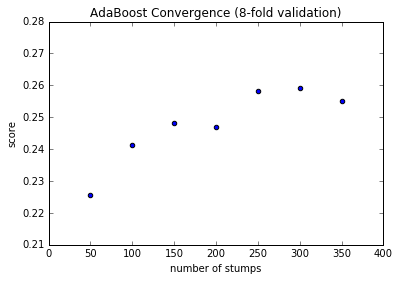
\includegraphics[scale=0.5]{ada-convergence.png}
        \label{fig:ada-convergence}
        \caption{The slow rise as the number of learners increases indicates that AdaBoost is either converging or will take too many estimators to approach a decent accuracy.}
    \end{minipage}
    \hfill
    \begin{minipage}[b]{0.4\textwidth}
        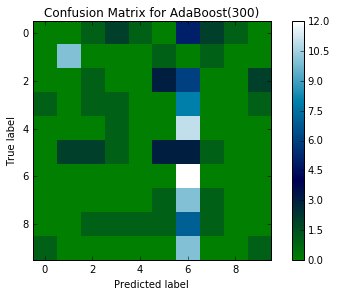
\includegraphics[scale=0.5]{ada-confusion.png}
        \label{fig:ada-confusion}
        \caption{This confusion matrix suggests that AdaBoost on decision stumps will not
        work for this problem, as the weighting pathologically emphasizes a certain label, preventing much improvement over all 10 labels.}
    \end{minipage}
    
    \label{fig:fv33}
\end{figure}

\subsubsection{Majority Voting over Features}\label{majority-features}

Code: \texttt{multi-feature-voter.ipynb}. 

We attempted to improve the accuracy of our methods by using a majority-voting ensemble over the different features, in hopes that different features could inform different genre classifications orthogonally. Concatenating the features and applying a simple classifier alone only worsened performance. This is probably due to the varying levels of predictability each of the features had. In classifiers such as SVM, adding in less predictive features may hurt performance because it results in poorer choices for support vectors that don't generalize.

For the majority algorithm, we used an \texttt{mfcc} FV(3,3), \texttt{eng}, \texttt{hcdf}, and \texttt{brightness} SVMs as well as \texttt{zerocross} and \texttt{roughness} based Random Forests.

Each of these had optimal parameters selected from previous cross validation runs (see previous two sections above). Cross-validating the soft majority-vote (which sums the probabilities assigned to each label and chooses the largest value) on 8 folds yielded 0.49 accuracy, which improved on most of the classifiers but only dragged the \texttt{mfcc} SVM down. 

\subsubsection{Majority Voting over Algorithms}

Code: \texttt{fv-voter.ipynb}.

Observing that Softmax, mSVM, Random Forest, and Nearest Neighbors
each had good performance on FV(3, 3),
Thus, we used a soft-voting algorithm that combined these four
algorithms with equal weight.
The hyper-parameters we used were the optimized ones that we had
discovered when we ran each of the algorithms individually.
This method overfits,
as we were using our knowledge that these particular methods
work well and our computed hyperparameters from the data set
to create this voter which would once again run on the same data.
However, this overfitting was unavoidable, and we believe
it should not have caused too much overfitting.
We also note that this voter used soft-voting, meaning that
it combined the probability distribution vectors and took
the genre with highest probability rather than taking
the maximum among votes.
We obtained $69.5\%$ accuracy with this method using 8-fold cross validation, 
which only slightly exceeded our mSVM's accuracy on the same data.
We also ran hard-voting out of curiosity, and got just under $69\%$ accuracy with it.
This tells us that most of these methods are likely misclassifying 
in similar ways, as otherwise we would expect that the voter would
have out performed the individual algorithms by a greater margin.

\subsubsection{Convolutional Neural Network}\label{cnn}

Code: \texttt{CNN.ipynb}. We also attempted a 3-layer CNN using \texttt{TensorFlow} \cite{tensorflow2015-whitepaper}. Unfortunately, this took a whole night to train and lead to only 49\% accuracy, likely due to overfitting (it had no error on the training set). It would be interesting to investigate other topologies, but this was not feasible in the time constraints for this project.

\subsubsection{Binary-Tree SVM}

Code: \texttt{fv-msvm.ipynb} (at the bottom).
We had an idea that perhaps the fisher vectors will cluster in such
a way that some groups of genres hang close together with wide
gaps between such groups.
Thus, we coded up a SVM-binary-search-tree algorithm that
found the best partition of the set of 10 genres $G$ into 
subsets $G_0, G_1$ such that the linear separator between them
has maximum margin over all such partitions ($G_0$ and $G_1$ could be
of any non-zero size), and then recursively proceeded until
all the leaves were singleton sets.
This exponential procedure was fast enough to run as there are only
10 genres (we consider every possible subset of genres for 0/1-classification).
However, unfortunately every partition we made separated precisely
one genre from the rest of the genres,
and thus essentially regressed into one-vs-rest mSVM, but performed worse than the ovo SVM.
The performance only worsened when we tried to impose
that our decision tree made partitions for which both sides of the 
partition had more than one genre where possible.


\end{document}